% CVPR 2026 Paper Template; see https://github.com/cvpr-org/author-kit
%
% clashbot final report, CAP 6938 AI Knowledge Systems (UCF), ported from the IEEE version
% (docs/report/clashbot_report.tex) to the CVPR 2026 author kit required by the instructor.
% Compile: pdfLaTeX + BibTeX on Overleaf (root file main.tex), or locally: tectonic -X compile main.tex
% Page rule (CVPR): at most eight pages excluding references.
%
% Source convention: every number carries a "% src:" comment naming the file it was copied from.
%   CMA = docs/research/course_mapping_audit.md       PBA = docs/research/packaging_and_benchmarks_audit.md
%   PBC = docs/research/prior_bots_comparison.md      CGA = docs/research/course_gap_analysis.md
%   BM  = docs/data/BENCHMARKS.md   SA = docs/data/stats_audit_v1.md   STATUS = docs/mac/STATUS.md
%   D-nnn = docs/decisions/DECISIONS.md   CC = docs/data/context_conflict_v1.md   AR = docs/data/answer_rules_v1.md
%   VP = docs/data/vs_pro_v1.md   LAT = docs/data/latency_v2.md
% Revision 2 (2026-11-07): every number once tagged [pre-merge] was re-checked against the merged docs/data
% files (MAC-AP, MAC-AR) and the tag removed.
% Revision 3 (2026-11-07 night): vs_pro_v1 is final (all 24 usable test games, generated 2026-11-08T02:31:35Z); the
% Training Camp trial is filled. TRIAL = the user's recorded results of the 10 trial battles (2026-11-07 evening,
% scripts/demo.sh --live, frozen code D-051) as relayed for revision 3; LOG = session log runs/demo/20261107-213709
% (battles.jsonl, decisions.jsonl; 9 of 10 battles logged); BL = docs/plans/BACKLOG_post_showcase.md (W1-W12).
% Revision 4 (2026-11-09): CVPR port. Two benchmark subsections are reserved as \TODO placeholders in
% sec/5_experiments.tex (Decision models; Retrieval methods for the KB and the KG).
% Revision 5 (2026-11-09): both placeholders filled (MAC-AU) from docs/data/decision_models_v1.{md,json} and
% docs/data/retrieval_methods_v1.{md,json} (the only sources of the new numbers; Sonnet row = claude-sonnet-5-5-long).
% The former Table kg part (b) (E6 test) is folded into Table retrmethods (b), which repeats its test numbers exactly;
% its val column moved to the E6 text. Older text condensed to stay within eight pages; no result dropped.

\documentclass[10pt,twocolumn,letterpaper]{article}

%%%%%%%%% PAPER TYPE  - PLEASE UPDATE FOR FINAL VERSION
\usepackage{cvpr}              % To produce the CAMERA-READY version (shows the author; no line numbers)
% \usepackage[review]{cvpr}      % To produce the REVIEW version
% \usepackage[pagenumbers]{cvpr} % To force page numbers, e.g. for an arXiv version

% Import additional packages in the preamble file, before hyperref
%% This file contains a number of tweaks that are typically applied to the main document.
%% They are not enabled by default, but can be enabled by uncommenting the relevant lines.

%%
%% Inline annotations; for predefined colors, refer to "dvipsnames" in the xcolor package:
%% https://tinyurl.com/overleaf-colors
%%
\newcommand{\red}[1]{{\color{red}#1}}
\newcommand{\todo}[1]{{\color{red}#1}}
\newcommand{\TODO}[1]{\textbf{\color{red}[TODO: #1]}}
%%
%% disable for camera ready / submission by uncommenting these lines  
%%
% \renewcommand{\TODO}[1]{}
% \renewcommand{\todo}[1]{#1}

%%
%% work harder in optimizing text layout. Typically shrinks text by 1/6 of page, enable
%% it at the very end of the writing process, when you are just above the page limit
%%
% \usepackage{microtype}

%%
%% fine-tune paragraph spacing
%%
% \renewcommand{\paragraph}[1]{\vspace{.5em}\noindent\textbf{#1.}}

%%
%% globally adjusts space between figure and caption
%%
% \setlength{\abovecaptionskip}{.5em}


%%
%% Allows "the use of \paper to refer to the project name"
%% with automatic management of space at the end of the word
%%
% \usepackage{xspace}
% \newcommand{\paper}{ProjectName\xspace}

%%
%% Commonly used math definitions
%%
% \DeclareMathOperator*{\argmin}{arg\,min}
% \DeclareMathOperator*{\argmax}{arg\,max}

%%
%% Tigthen underline
%%
% \usepackage{soul}
% \setuldepth{foobar}
%% =====================================================================================
%% clashbot report additions (everything above this line is the unchanged CVPR 2026 kit file)
%% cvpr.sty already loads times, xcolor[dvipsnames], graphicx, amsmath, amssymb, booktabs,
%% natbib[numbers,sort&compress], caption, subcaption, url, enumitem and (at end of preamble)
%% cleveref, so none of them is loaded again here (no option clashes).
%% =====================================================================================
\usepackage{iftex}
\ifXeTeX % local tectonic builds only (Overleaf's pdfLaTeX skips this): XeTeX's default TU encoding has no
  % Times, so cvpr.sty's times package would silently fall back to Latin Modern. OT1 makes XeTeX use the same
  % Type 1 Times metrics as pdfLaTeX, so the local page count matches Overleaf.
  \usepackage[OT1]{fontenc}
\fi
\usepackage{array}
\usepackage{tikz}
\usetikzlibrary{arrows.meta}

\newcommand{\cb}{\textup{\textsc{clashbot}}}
\newcommand{\tw}[1]{\texttt{#1}}
\newcolumntype{L}[1]{>{\raggedright\arraybackslash}p{#1}}
% Tweak offered (commented out) by the kit above: tighter space between float and caption.
\setlength{\abovecaptionskip}{.5em}


% It is strongly recommended to use hyperref, especially for the review version.
% hyperref with option pagebackref eases the reviewers' job.
% Please disable hyperref *only* if you encounter grave issues,
% e.g. with the file validation for the camera-ready version.
%
% If you comment hyperref and then uncomment it, you should delete *.aux before re-running LaTeX.
% (Or just hit 'q' on the first LaTeX run, let it finish, and you should be clear).
\definecolor{cvprblue}{rgb}{0.21,0.49,0.74}
\usepackage[pagebackref,breaklinks,colorlinks,allcolors=cvprblue]{hyperref}

%%%%%%%%% PAPER ID
% Not a CVPR submission (course report): no paper ID, no conference header.
% \paperID and \confName are used by cvpr.sty only in review/rebuttal mode.
% \def\paperID{*****}
% \def\confName{CVPR}
% \def\confYear{2026}

%%%%%%%%% TITLE
\title{\cb{}: A Knowledge-Grounded LLM Agent That Plays Clash Royale\\in Real Time from Pixels}

%%%%%%%%% AUTHORS
\author{David Tyler Jackson (5298477)\\
University of Central Florida\\
{\normalsize CAP 6938 AI Knowledge Systems}\\
{\normalsize Instructor: Dr.\ Ser Nam Lim}
}

\begin{document}
\maketitle
\begin{abstract}
% src: CMA C1 (197 games, 10,923 states), C2 (KG v2 840/27,112), LOG (323 ms trial-session p50); SA sec. 1 (0.507, 0.482, 0.384); CC (E2); AR (E6); STATUS 2026-11-07 night (first win);
% src: docs/data/decision_models_v1.md (zero-shot on the same 766 test lines: claude-sonnet-5-5-long 0.364, Qwen3-14B 0.304, Claude Haiku 5.5 0.279)
We present \cb{}, a non-embedded agent that plays the real-time card game Clash Royale on an iPhone through macOS screen mirroring, pixels in and taps out, with every model on one laptop. Perception and a learned play/wait gate feed a candidate generator built from a lane simulator, hybrid retrieval over 10,923 states from 197 pro games and a knowledge graph (840 nodes, 27,112 edges); a fine-tuned 600M-parameter LLM picks one of at most four candidates. On held-out games it picks the pro's play 50.7\% of the time, against 25\% chance and 38.4\% for a placement prior. Zero-shot LLMs given the same prompt do far worse: Claude Sonnet 5.5 36.4\%, Qwen3-14B 30.4\%, Claude Haiku 5.5 27.9\%. Three results are negative: a tuned LightGBM ranker (48.2\%) statistically matches the LLM; corrupting the tool notes in its context leaves its accuracy unchanged; and answer rules mined from the pro games beat random but not card popularity. Open loop on 24 held-out pro games, the bot acts within 2\,s of 77.1\% of the pro's plays but picks the pro's card on only 17.1\%, largely because that card is in its perceived hand only 40\% of the time. % src: VP headline (77.1, 17.1, 40.1)
A live decision takes 323\,ms (median). The agent won one early Training Camp battle but lost all ten of a trial on frozen code (not significantly different from the prior agent KataCR's 1/20, Fisher $p=1.0$), which its logs trace to misread tower HP, no committed target tower, weak spell valuation and over-playing. % src: TRIAL; STATUS 2026-11-07 night (win in run 013441); BL W1, W2, W5, W8
\end{abstract}

\section{Introduction}
\label{sec:intro}

Clash Royale is a real-time, two-player phone card game: each player brings a hidden eight-card deck, holds four cards, and spends elixir (regenerating up to ten) to place troops, buildings and spells on an 18$\times$32-tile arena, for three minutes plus up to two of overtime~\cite{wu2025nonembedded}. % src: PBC sec. 1.1 (deck 8, hand 4, 3 + 2 min, 18 x 32 grid)
\cb{} is a \emph{non-embedded} agent~\cite{wu2025nonembedded}: with no game API, it reads the screen of an iPhone mirrored onto a Mac and clicks the mirrored window, the interface a human uses.

The task is hard for five measurable reasons. (i)~\emph{Real time}: perception targets 10\,fps (7.97\,fps in live run 111554); capture to click takes 323\,ms (median, live trial). % src: LOG (323 ms); CMA C7 (7.97 fps, run 20261107-111554)
(ii)~\emph{Partial, noisy observation}: the opponent's deck, hand and elixir are hidden, and the pro's recorded move passes our perceived-legality check on only 0.542--0.597 of states. % src: CMA A3 neuro-symbolic row (ranker_stats_v1.json pos_in_legal_rate)
(iii)~\emph{Structured actions plus timing}: card $\times$ lane $\times$ zone or hold (D-010), and pros deploy within 1\,s on about a fifth of seconds (dense act rate 0.204). % src: CMA B dense wait/act row
(iv)~\emph{Sparse supervision}: 197 pro games (about 12 match-hours, one creator), no reward or simulator, an opponent with level-15 cards. % src: CMA C1; D-047
(v)~\emph{Consumer hardware}: an Apple M5 laptop (32\,GB), no paid API. % src: CMA C3 (hardware); PBC sec. 4 (cost per game)

Following the course's retrieve-then-rank and agent-with-tools patterns~\cite{lim2026l11,lim2026l13,lim2026l15}, deterministic tools (a tactical engine with a lane simulator, hybrid retrieval over pro states and a knowledge graph) propose at most four candidate plays with short text notes, and a decision LLM fine-tuned on the pro games picks one; no tool picks the move (D-045; decision log D-001 to D-053). Contributions:
\begin{enumerate}
\item A non-embedded, two-speed agent live on iPhone Mirroring, all models local, with guarded demo tools (Sec.~\ref{sec:system}).
\item A knowledge layer (hybrid retrieval over 10,923 pro states, a two-version KG with lane-simulation edges and 3,620 mined pro answers, a tactical engine) rendered as context for a fine-tuned setwise LLM ranker. % src: CMA C1, C2, A1
\item A leakage-checked benchmark suite (Sec.~\ref{sec:exp}): options rebuilt after a leak (an option-key rule scored 0.852 on test), ten rankers with cluster-bootstrap CIs, ablations from retrieval to knowledge editing, and an open-loop comparison with the pro, negative results included. % src: D-037 (0.852 test)
\item Live Training Camp evaluation: 13 recorded runs (931 logged decisions) with one win, then a 0--10 trial on frozen code, diagnosed from the logs (Sec.~\ref{sec:live}, \ref{sec:disc}). % src: CMA C6; STATUS 2026-11-07 night; TRIAL; BL
\end{enumerate}
The bot plays only Training Camp and friendly battles, never ranked matches against people (D-031, D-050).

% ---------------------------------------------------------------------------------------------
\begin{figure*}[t]
\centering
\resizebox{\textwidth}{!}{%
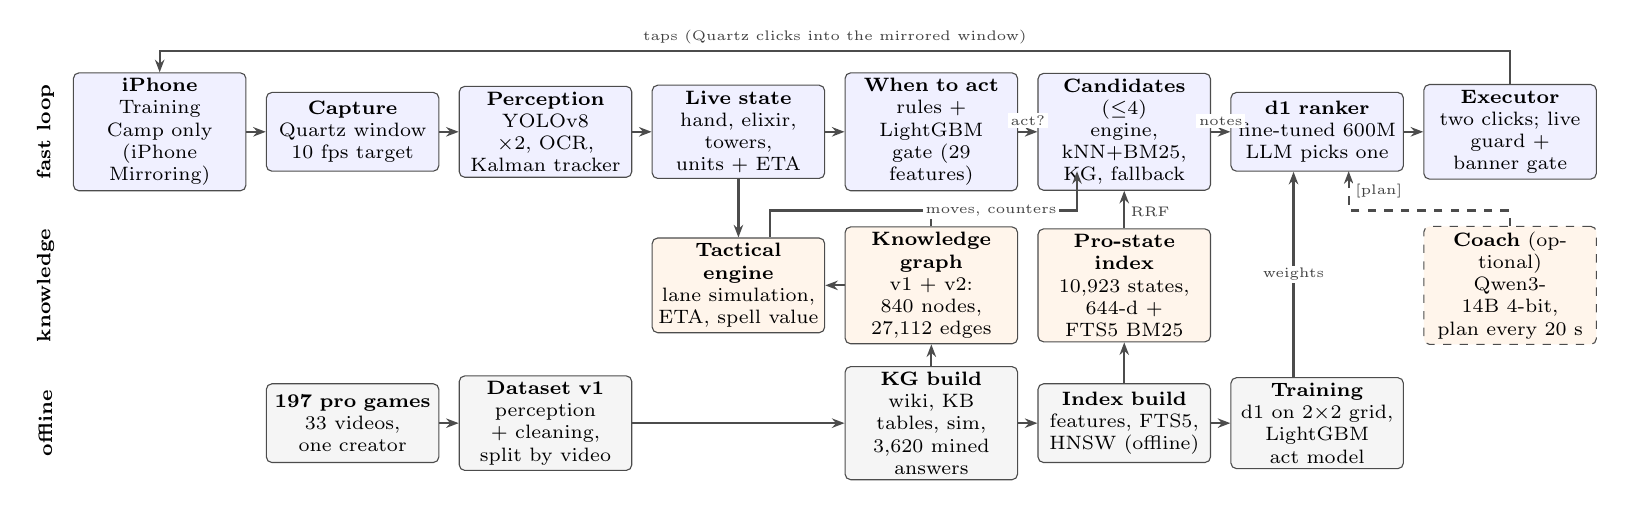
\begin{tikzpicture}[
  box/.style={draw=black!70, rounded corners=2pt, align=center, font=\scriptsize,
              text width=2.05cm, minimum height=1.0cm, inner sep=2pt, fill=white},
  fast/.style={box, fill=blue!6},
  know/.style={box, fill=orange!8},
  off/.style={box, fill=black!4},
  arr/.style={-{Stealth[length=1.6mm]}, thick, draw=black!70},
  lab/.style={font=\tiny, text=black!75, fill=white, inner sep=1pt}]
% row 1: fast loop
\node[fast] (phone) at (0,0)     {\textbf{iPhone}\\Training Camp only\\(iPhone Mirroring)};
\node[fast] (cap)   at (2.45,0)  {\textbf{Capture}\\Quartz window\\10 fps target};
\node[fast] (per)   at (4.9,0)   {\textbf{Perception}\\YOLOv8 $\times$2, OCR,\\Kalman tracker};
\node[fast] (st)    at (7.35,0)  {\textbf{Live state}\\hand, elixir, towers,\\units + ETA};
\node[fast] (gate)  at (9.8,0)   {\textbf{When to act}\\rules + LightGBM\\gate (29 features)};
\node[fast] (cand)  at (12.25,0) {\textbf{Candidates} ($\le$4)\\engine, kNN+BM25,\\KG, fallback};
\node[fast] (d1)    at (14.7,0)  {\textbf{d1 ranker}\\fine-tuned 600M\\LLM picks one};
\node[fast] (ex)    at (17.15,0) {\textbf{Executor}\\two clicks; live\\guard + banner gate};
% row 2: knowledge layer
\node[know] (eng)   at (7.35,-1.95)  {\textbf{Tactical engine}\\lane simulation,\\ETA, spell value};
\node[know] (kg)    at (9.8,-1.95)   {\textbf{Knowledge graph}\\v1 + v2: 840 nodes,\\27,112 edges};
\node[know] (idx)   at (12.25,-1.95) {\textbf{Pro-state index}\\10,923 states,\\644-d + FTS5 BM25};
\node[know, dashed] (coach) at (17.15,-1.95) {\textbf{Coach} (optional)\\Qwen3-14B 4-bit,\\plan every 20 s};
% row 3: offline
\node[off] (vid)    at (2.45,-3.7)  {\textbf{197 pro games}\\33 videos,\\one creator};
\node[off] (ds)     at (4.9,-3.7)   {\textbf{Dataset v1}\\perception + cleaning,\\split by video};
\node[off] (kgb)    at (9.8,-3.7)   {\textbf{KG build}\\wiki, KB tables, sim,\\3,620 mined answers};
\node[off] (idxb)   at (12.25,-3.7) {\textbf{Index build}\\features, FTS5,\\HNSW (offline)};
\node[off] (tr)     at (14.7,-3.7)  {\textbf{Training}\\d1 on 2$\times$2 grid,\\LightGBM act model};
% row labels
\node[font=\scriptsize\bfseries, rotate=90] at (-1.45,0)     {fast loop};
\node[font=\scriptsize\bfseries, rotate=90] at (-1.45,-1.95)  {knowledge};
\node[font=\scriptsize\bfseries, rotate=90] at (-1.45,-3.7) {offline};
% fast-loop arrows
\draw[arr] (phone) -- (cap);
\draw[arr] (cap) -- (per);
\draw[arr] (per) -- (st);
\draw[arr] (st) -- (gate);
\draw[arr] (gate) -- node[lab, above=1pt] {act?} (cand);
\draw[arr] (cand) -- node[lab, above=1pt] {notes} (d1);
\draw[arr] (d1) -- (ex);
\draw[arr] (ex.north) -- ++(0,0.42) -| node[lab, pos=0.25, above=1pt] {taps (Quartz clicks into the mirrored window)} (phone.north);
% knowledge-layer arrows
\draw[arr] (st.south) -- (eng.north);
\draw[arr] (kg.west) -- (eng.east);
\draw[thick, draw=black!70] (kg.north) -- (9.8,-1.0);
\draw[arr] ([xshift=4mm]eng.north) |- (11.65,-1.0) -- node[lab, pos=0.0, left=6pt] {moves, counters} (11.65,-0.5);
\draw[arr] (idx.north) -- node[lab, right=1pt, pos=0.45] {RRF} (cand.south);
\draw[arr, dashed] (coach.north) |- (15.1,-1.0) -- node[lab, pos=0.5, right=1pt] {[plan]} (15.1,-0.5);
% offline arrows
\draw[arr] (vid) -- (ds);
\draw[arr] (ds) -- (kgb);
\draw[arr] (kgb) -- (idxb);
\draw[arr] (idxb) -- (tr);
\draw[arr] (kgb) -- (kg);
\draw[arr] (idxb) -- (idx);
\draw[arr] ([xshift=-3mm]tr.north) -- node[lab, pos=0.5] {weights} ([xshift=-3mm]d1.south);
\end{tikzpicture}}
\caption{Two-speed architecture (D-007). The fast loop runs on every decision (323\,ms p50 capture to click in the live trial); tools in the knowledge layer only propose candidates and write notes, and the fine-tuned d1 LLM picks the move (D-045). The coach is optional and off by default. Every decision is logged and can be replayed in the dashboard (Fig.~\ref{fig:dashboard}).}
\label{fig:pipeline}
\end{figure*}
% src (figure numbers): LOG (323 ms), C2 (840 / 27,112), C1 (197 games, 33 videos, 10,923 x 644), C3/B (Qwen3-14B coach, 20 s period), act_gbdt_v1.md (29 features), CMA C2 extras (3,620 answers)

\section{Related Work}
\label{sec:related}

\emph{Game agents.} AlphaStar~\cite{vinyals2019alphastar} and OpenAI Five~\cite{berner2019dota} reached expert level through game APIs and self-play, unavailable for a phone game. The closest work, KataCR~\cite{wu2025nonembedded}, is a non-embedded Clash Royale agent (YOLOv8 detectors, OCR, an offline-RL StARformer policy in the Decision Transformer formulation~\cite{chen2021dt}) that won 1 of 20 Training Camp games (Table~\ref{tab:prior}); we reuse its detector weights~\cite{wu2024katacr} and protocol. Claude Royale~\cite{houseworth2025claudeRoyale} runs Claude Haiku agents at about 7\,s per decision on the human ladder. % src: PBC sec. 1.3, 2.1, 2.2
\emph{LLM agents and ranking.} ReAct, Reflexion and LATS~\cite{yao2023react,shinn2023reflexion,zhou2024lats} spend seconds per step on reasoning, reflection or search; a real-time budget rules out generation in the fast loop, so our LLM is a setwise reranker~\cite{zhuang2024setwise,sun2023rankgpt} over tool proposals, as in two-stage recommender serving~\cite{yi2019twotower,lim2026l13}. Fine-tuning an LM to choose among items follows TALLRec and P5~\cite{bao2023tallrec,geng2022p5}, graph facts in the context follow GraphRAG~\cite{edge2024graphrag}, and deciding when to consult the model follows adaptive retrieval~\cite{jiang2023flare,jeong2024adaptiverag}.

\section{System}
\label{sec:system}

Fig.~\ref{fig:pipeline} shows the two-speed design (D-007). \cb{} is an agent with tools~\cite{lim2026l15}, but unlike a ReAct agent~\cite{yao2023react} its LLM does not call them: the tools run on every decision, propose candidate plays and write notes, and only the fine-tuned d1 ranker picks one (D-045). An optional slow loop (Qwen3-14B, 4-bit~\cite{qwen2025qwen3}) serves as a long-horizon planner beside this fast actor~\cite{lim2026l16}: it rewrites a three-line plan every 20 game seconds, never picks a move, and was used in one live run (21 plans, 5.98/6.86\,s p50/p95). The default live path calls no generative LLM. % src: CMA B coach row (run 20261106-133529)

\subsection{Perception and live state}
Quartz window capture grabs the iPhone Mirroring window (632$\times$1392 pixels, 22--38\,ms per grab). % src: STATUS 2026-11-03 Wave 4
Two YOLOv8 detectors~\cite{jocher2023yolov8} with KataCR's weights~\cite{wu2024katacr} (87.8\,MB each) run on the M5 GPU (100.5\,ms per call), RapidOCR~\cite{rapidai2021rapidocr} reads the clock and deploy labels in the background, a template matcher reads the hand slots (33.1\,ms) only when a slot crop changes (D-038), and a Kalman tracker~\cite{kalman1960} follows units. % src: CMA C3, C7
The live state holds both sides' elixir, our hand, towers, the opponent's seen cards and each unit's time to reach a tower (ETA); ETA from card speed and attack range instead of the raw track cut its median absolute error from 1.49\,s to 0.30\,s and raised the share within 1\,s from 34\% to 80\% (384 frames, 11 arrivals, one video). % src: docs/data/eta_eval_v1.md (= runs/smoke/AL/eta.md; BM sec. 10)
It also built the dense training data (D-040), so live and offline features match.

\subsection{Data, knowledge graph and retrieval}
\textbf{Data.} A scraper built a knowledge base from the wiki; 197 games from 33 videos of one professional creator were perceived and cleaned into 10,923 states (6,901 plays, 3,539 key moments, 483 periodic samples), with bad fields repaired and flagged, never deleted (D-011; 2,165 states lack a known placement). % src: README.md (Phase 1, scraper); CMA C1 (MANIFEST, CLEANING_REPORT_v1.md)
Splits are by video (SHA-1 order, 70/15/15), so no game spans splits (the contamination concern of RETRO~\cite{borgeaud2022retro}): train/val/test hold 23/5/5 videos, 142/27/28 games, 7,693/1,574/1,656 states and 3,641/761/766 ranker lines. A second pass at one state per second ($\sim$17\,h on the M5) gave 29,036/5,560/5,279 dense play/wait lines (does the pro deploy within 1\,s?); 3,654 pro-advice documents complete the store. % src: CMA C1, A2 RETRO row; PBA 1.2 (17 h)
% src: CMA C1 (splits, ranker set, dense set, documents), C2 (KG v1/v2 counts, sim 8,951, answers 287, extras)

\textbf{Knowledge graph.} Game knowledge is stored as a typed graph~\cite{cap6938L05}. KG v1 (590 nodes, 12,030 edges, 12 relations) holds wiki COUNTERS and SYNERGY relations, deck membership and 129 mined ANSWERED\_BY edges. KG v2 (D-048; 840 nodes, 27,112 edges, 19 relations) adds a game model: per-level stats for 126 cards (1,734 rows, opponents assumed at level 15), 8,951 STOPS, KILLS and PULLS edges from the lane simulator, 3,620 mined answer events (the opponent plays $X$; the pro's first defensive play within 8\,s is $Y$) aggregated by support-counted rule mining~\cite{lajus2020amie3,liu2022tlogic} into 287 rules with held rates, placement offsets and timing, 234 situation nodes, 450 PLAYED\_AFTER sequences, deck co-occurrence, and role-similarity transfer for our cards without pro data; an opponent-deck model completes the hidden deck from the cards seen. % src: CMA C2, A3; answer window 8 s: CGA sec. 8, answer_rules_v1.md
Live, the graph supplies the engine's answer prior, pro placement offsets ($n\ge5$), an elixir reserve for predicted air cards, a counter channel for candidates, and up to three \tw{KG:} lines in d1's context, graph facts given to the ranker as in GraphRAG~\cite{edge2024graphrag,lim2026l12} (Fig.~\ref{fig:dashboard}). % src: CMA B (KG v2 facts row, example line); STATUS 2026-11-06 evening

\textbf{Retrieval.} Each state is a fixed-length, hand-built (not learned~\cite{lim2026l02}) 644-d structured vector (3 scalars, 5 phase values, five 120-d card blocks for hand, deck, opponent deck and both sides' recent plays, 6 tower, 24 field and 6 threat values) plus a text rendering indexed by SQLite FTS5 BM25~\cite{robertson2009bm25}. Exact dot-product kNN and BM25 lists are fused by reciprocal rank fusion ($k=60$)~\cite{cormack2009rrf,cap6938L09}, and the neighbours vote for the plays they contain. A 384-d bge-small text embedder channel~\cite{xiao2023cpack,lim2026l03} and an approximate HNSW index~\cite{malkov2020hnsw,cap6938L09}, compared with exact search, were evaluated offline only (Sec.~\ref{sec:retr}). % src: CMA A1 (644-d breakdown, RRF k = 60, HNSW offline only, text channel not integrated)

\subsection{Tactical engine, timing and the d1 ranker}
\textbf{Tactical engine.} The engine (1,750 lines; roles for 122 cards) lists enemy pushes, estimates each push's tower damage by lane simulation over per-level stats, and proposes placed answers with reasons (a lone level-15 Balloon deals 3,162 tower HP unanswered, 351 with a Musketeer behind the tower, 0 with a Tesla pull). It values spells by kills (a Zap needs two kills and value 2.5), leads them by flight time, keeps buildings inside a pull box, and tracks elixir trades and offence windows; d1 reads its analysis as \tw{tactics:} lines and per-option notes (D-042). % src: CMA B (1,750 lines, 122 cards, balloon 3,162/351/0); STATUS MAC-AM merged (spell bar, lead, tesla box)

\textbf{When to act.} A reactive policy (modes defend, leak, punish, counter, spell, save, none; D-041) holds by default and filters candidates by mode. A LightGBM~\cite{ke2017lightgbm} model on 29 features predicts whether a pro would deploy within 2\,s (threshold 0.47, 0.05\,ms per call); in the live \emph{fast} policy rules override it in defend, counter, spell and leak, and save and none always hold. This gate is our adaptive trigger~\cite{jiang2023flare,jeong2024adaptiverag,lim2026l12}: it decides when the LLM is consulted at all. % src: CMA sec. 0 (when to act), B (act model 0.045 ms)

\textbf{Candidates and d1.} The generator returns at most four plays (up to two engine moves, then retrieval votes, KG v1 counter scores with weight 0.5, legal fallbacks). Hard symbolic constraints~\cite{cap6938L07} then filter them: the card must be in the read hand with enough elixir and a legal placement, the policy's mode must allow the play, and fallbacks are held below 9.5 elixir. % src: CMA sec. 0 (candidates, filters)
d1 is Liquid AI's d1-omni-600M~\cite{liquidai2026d1omni}, a 16-layer trunk whose head emits one logit per option marker, scoring all options in one pass (setwise LLM reranking~\cite{zhuang2024setwise,sun2023rankgpt,cap6938L10}). Zero-shot it is at chance (Sec.~\ref{sec:ranker}), so, as TALLRec and P5 fine-tune a language model as a recommender~\cite{bao2023tallrec,geng2022p5,lim2026l14}, we fine-tuned the full text path (313.6M parameters, fp32 on MPS) with a softmax cross-entropy over the options: \tw{d1-ft-joint} on states alone (3 epochs, 13,241\,s), then the live \tw{d1-ft-joint-tac} with tactics lines and notes (2 epochs, 4,554\,s, peak 22.75\,GB). % src: docs/plans/MAC-T_d1_finetune.md sec. 0 (16 layers, logit per option marker); CMA C4, A2 TALLRec row
Live, d1 takes 92.7/174.7\,ms (p50/p95) and runs only when $\ge$2 candidates survive (119/279 plays, three pre-trial runs). % src: CMA C6, sec. 0

\textbf{The option-set shortcut (D-037).} Our first training set built three negatives per pro play (a neighbour's play, the same card elsewhere, another card at the same spot), so the positive was always the option sharing its card with one option and its placement with another: a rule reading only the option keys scored 0.848/0.853/0.852 on train/val/test. In the rebuilt 2$\times$2 grid \{pro card, second possible card\} $\times$ \{pro placement, second legal placement\} every option shares its card and placement with exactly one other, so the key-only rule scores 0.25 by construction while the negatives stay hard (\cf RAFT's distractors~\cite{zhang2024raft,lim2026l11}); a random second placement removed a fixed lane order (lane-only rule 0.31 $\rightarrow$ 0.272). % src: D-037; ranker_stats_v1.json via CMA A2 (lane-only 0.2722 test)

\subsection{Executor, safety and demo tooling}
The executor sends two calibrated Quartz clicks (card slot, then tile) 50\,ms apart (execute stage 181\,ms at the median in the trial), tracks own elixir, detects failed taps and cools a failed card down for 2\,s. Two independent switches, the \tw{--live} flag and \tw{CLASHBOT\_ALLOW\_LIVE=1}, gate every tap, checked at construction and before every action (D-031). % src: CMA C7 (execute 183.3); STATUS 2026-11-05 night (MAC-AC C2); D-031
The demo launcher (about 10\,s to load) taps only in battles whose opponent banner reads ``Trainer''; an unreadable banner counts as not Training Camp (D-050). It read 411 of 412 recorded banners and 5 of 5 battles correctly. The dashboard (Fig.~\ref{fig:dashboard}) replays or follows a run decision by decision; logging costs about 0.03\,ms per decision. % src: STATUS 2026-11-07 showcase prep (MAC-AN, MAC-AO)

\begin{figure}[t]
% full-resolution screenshot (1700 x 2000 px): zoom in the PDF for detail; caption set beside it to save height
\begin{minipage}[c]{0.6\columnwidth}
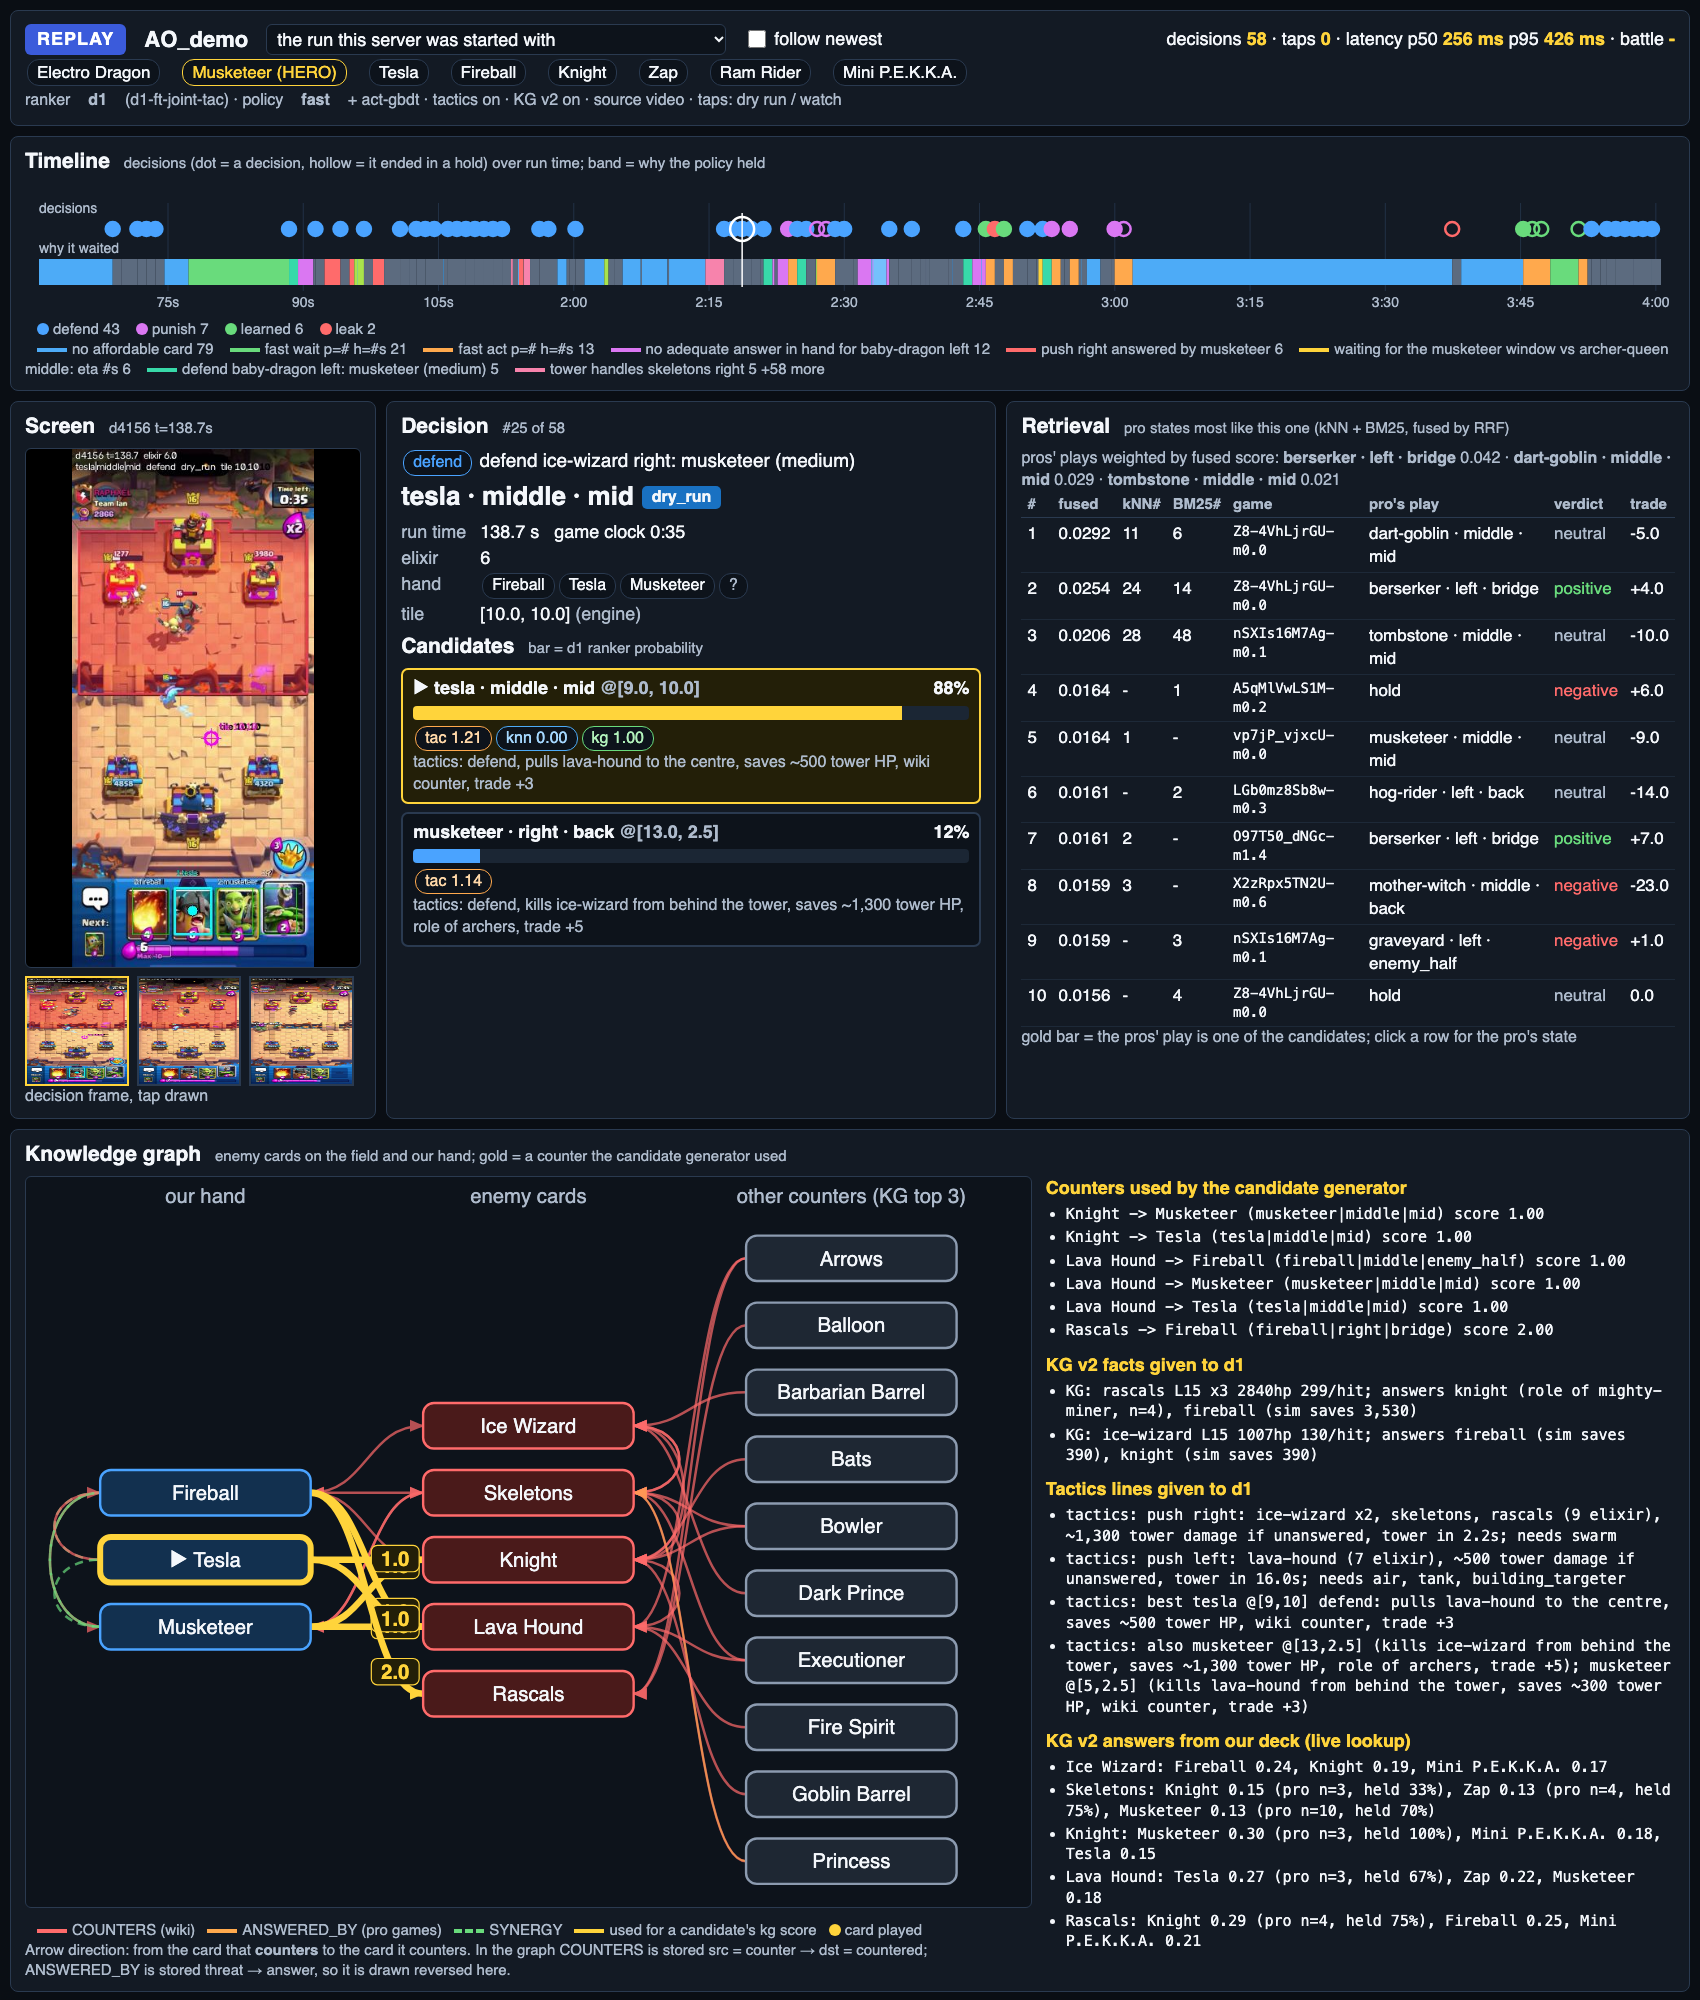
\includegraphics[width=\linewidth]{figs/dashboard.png}
\end{minipage}\hfill
\begin{minipage}[c]{0.37\columnwidth}
\captionsetup{justification=raggedright,singlelinecheck=false}
\caption{Decision dashboard on a video dry run. Top: timeline of decisions and hold reasons. Middle: decision frame; two candidates with d1 probabilities (Tesla 88\%) and the engine, kNN and KG scores behind them; the ten pro states retrieved by kNN+BM25 with RRF. Bottom: KG subgraph (our hand, enemy cards, counters used) and the \tw{KG:} and \tw{tactics:} lines d1 read.}
\label{fig:dashboard}
\end{minipage}
\end{figure}

\section{Course Concepts in the System}
\label{sec:course}

Table~\ref{tab:course} maps each course block to what is built, where it runs and the number that tests it; Sec.~\ref{sec:disc} draws together the four course lessons that recur in the results.

\begin{table*}[t]
\caption{Course techniques in \cb{}. Use: live = default live path; off = offline evaluation or a flag only. Test split unless noted; numbers from Sec.~\ref{sec:exp}.}
\label{tab:course}
\centering\scriptsize
\setlength{\tabcolsep}{3pt}
\begin{tabular}{@{}L{1.8cm}L{4.55cm}L{4.55cm}L{5.0cm}l@{}}
\toprule
Block & Technique & Where in \cb{} & Evidence & Use\\
\midrule
Retrieval
 & BM25~\cite{robertson2009bm25} + RRF ($k{=}60$)~\cite{cormack2009rrf} & FTS5 channel fused with structured kNN & hit@10 0.160 fused vs 0.136 kNN alone & live\\
L8--10~\cite{cap6938L08,cap6938L09,cap6938L10}
 & HNSW~\cite{malkov2020hnsw} vs exact search & index over 10,923 state vectors & ef 40: recall@10 0.978, 0.31 vs 1.51\,ms & off\\
 & Pre- vs post-filtering & deck and phase filters & pre-filter pool empty 88.9\%; post@10 50\%/87\% & off\\
 & Setwise LLM reranking~\cite{zhuang2024setwise,sun2023rankgpt} & d1 scores all ($\le$4) options in one pass & 0.507 fine-tuned vs 0.221 zero-shot (chance 0.25) & live\\
Dense repr.
 & Fixed-length state vectors & 644-d hand-built vector & structured kNN hit@10 0.136 & live\\
L2--4~\cite{lim2026l02,lim2026l03}
 & Small text embedder~\cite{xiao2023cpack} & 384-d bge-small channel & adds $\sim$20\,ms, hit@10 0.143: not integrated & off\\
RAG
 & Parametric-memory limit~\cite{mallen2023popqa} & engine, retrieval and KG notes in context & zero-shot d1 at chance; by key popularity: Fig.~\ref{fig:popularity} & live\\
L11--12~\cite{lim2026l11,lim2026l12}
 & Distractor training (RAFT)~\cite{zhang2024raft} & 1 gold + 3 hard options on a 2$\times$2 grid & option-key shortcut 0.852 $\rightarrow$ 0.250 & train\\
 & Graph facts in context (GraphRAG)~\cite{edge2024graphrag} & up to 3 \tw{KG:} lines per decision & retrain on them: $-$2.2 pts [$-$4.7, +0.5] & live\\
 & Adaptive trigger~\cite{jiang2023flare,jeong2024adaptiverag} & play/wait gate decides when d1 is called & bal.\ acc.\ 0.607 LightGBM vs 0.509 rules ($h{=}2$\,s) & live\\
 & Abstention scoring (CRAG)~\cite{yang2024cragbench} & hold when d1's top probability $<$ 0.483 & utility 0.104 vs 0.013 answering all & off\\
Rec.\ systems
 & LM as recommender, full fine-tune~\cite{bao2023tallrec,geng2022p5} & d1-omni-600M, 313.6M trained parameters & val/test 0.547/0.507 & live\\
L13--14~\cite{lim2026l13,lim2026l14}
 & Feature rankers~\cite{wang2021dcnv2,burges2010lambdamart}; tuned baselines~\cite{rendle2020ncfvsmf} & logreg, LambdaRank, DCN-V2; 783 features & d1 $-$ LightGBM: +2.5 pts [$-$1.4, +5.9] & off\\
 & Sequential rec.\ (SASRec)~\cite{kang2018sasrec} & opponent next-card prediction & acc@1 0.222 vs copy-frequency 0.243 & off\\
KG
 & Typed KG feeding decisions & v1 590/12,030; v2 840/27,112, 19 relations & opp.-deck recall 0.234 vs popularity 0.130 ($k{=}1$) & live\\
L5--7~\cite{cap6938L05,cap6938L06C,cap6938L07}
 & KGE~\cite{bordes2013transe,yang2015distmult,trouillon2016complex,sun2019rotate}, audit protocol~\cite{ruffinelli2020olddog,sun2020reevaluation} & held-out COUNTERS triples, PyKEEN~\cite{ali2021pykeen} & RotatE MRR 0.159 vs popularity 0.110 & off\\
 & Rule mining with support~\cite{lajus2020amie3,liu2022tlogic} & 287 threat $\rightarrow$ pro-answer rules (8\,s) & hit@1 0.154; popularity 0.169, random 0.128 & live\\
 & Temporal copy mechanism~\cite{zhu2021cygnet} & copy-frequency over PLAYED\_AFTER & acc@1 0.243, beats SASRec & off\\
 & Neuro-symbolic hard constraints (L7) & legality filter, safety rules, lane simulation & pros' own play legal on 0.542--0.597 of states & live\\
Agents
 & Agent with tools~\cite{yao2023react}; one decision LLM & engine, retrieval, KG propose; d1 decides & 13 runs, 931 logged decisions, 746 taps & live\\
L15--16~\cite{lim2026l15,lim2026l16}
 & Guarded execution & two-switch guard, banner gate, decision logs & taps landed 75/84, 78/95; trial 0/10 wins & live\\
 & Trajectory-level evaluation~\cite{yao2025taubench} & open loop vs the pro on held-out videos & pro plays met $\pm$2\,s 77.1\% (null 68.9\%) & off\\
Knowl.\ updating
 & Editing criteria~\cite{yao2023editingsurvey}; non-parametric edit~\cite{mitchell2022serac} & patch-versioned fact store & reliability 1.000; portability 1.000 vs 0.067 & off\\
L17--18~\cite{lim2026l17,lim2026l18}
 & Knowledge conflicts~\cite{wu2024clasheval,xie2024chameleon} & corrupted tool notes (E2) & poisoned-note follow-rate 0.044; $-$0.4 pts & off\\
 & CAD/AdaCAD~\cite{shi2024cad,wang2025adacad}; stale facts & contrastive decoding; pre-patch down-weight & CAD no gain; stale hits 0.124 $\rightarrow$ 0.002 & off\\
\bottomrule
\end{tabular}
\end{table*}
% src (Table course): retrieval_ablation_v1.md (0.160, 0.136, 0.978, 0.31, 1.51, 88.9%, 50%/87%, 0.143); SA sec. 1/2/4 (0.507, 0.221, 0.547, -2.2, +2.5, 0.104/0.013); D-037 (0.852);
%   act_gbdt_v2.md (0.607 vs 0.509); CMA A2 (313.6M), A3 (0.542-0.597), C2, C6; next_card_v1.md (0.222, 0.243); opp_model_v1.md (0.234 vs 0.130);
%   kge_link_prediction_v1.md (0.159, 0.110); answer_rules_v1.md (0.154, 0.169, 0.128); BM sec. 11 (75/84, 78/95); edit_eval_v2.md = edit_eval_v1.md;
%   CC replicate joint_tac_v2, test (C3 follow-rate 0.044, delta -0.004; CAD a tuned on val = 0); VP headline (77.1%, null 68.9%); TRIAL (0/10)

\section{Experiments}
\label{sec:exp}

\emph{Setup.} Offline numbers come from the frozen decision code (D-051, commit \tw{66917e7}), with older outputs re-run. Ranker evaluations use 761 val and 766 test lines from 26 and 27 held-out games. CIs are percentile intervals from 10,000 cluster-bootstrap resamples of whole games (seed 20261107), paired across models; exact McNemar $p$, which treats lines as independent, is the optimistic test. Thresholds, ensemble weights and feature-ranker configurations are chosen on val, so test is the clean column. % src: BM header; SA header

\subsection{Ranking the pro's play}
\label{sec:ranker}

\begin{table}[t]
\caption{4-way pick-the-pro-play accuracy (chance 0.25) with 95\% cluster-bootstrap CIs. ``Notes'' = tactics lines and per-option notes.}
\label{tab:ranker}
\centering\scriptsize
\setlength{\tabcolsep}{3pt}
\begin{tabular}{@{}lll@{}}
\toprule
Model & Val & Test\\
\midrule
\multicolumn{3}{@{}l}{\emph{Leak check and simple baselines}}\\
option-key rule, old options / 2$\times$2 grid & 0.853 / 0.250 & 0.852 / 0.250\\
random & 0.230 [0.207, 0.254] & 0.252 [0.218, 0.284]\\
popularity of the key & 0.468 [0.412, 0.516] & 0.325 [0.280, 0.374]\\
placement prior & 0.493 [0.430, 0.547] & 0.384 [0.337, 0.431]\\
\multicolumn{3}{@{}l}{\emph{Feature rankers, 783 features (seed 0)}}\\
logistic regression & 0.543 [0.492, 0.586] & 0.470 [0.423, 0.512]\\
LightGBM LambdaRank & 0.565 [0.520, 0.604] & 0.482 [0.448, 0.515]\\
\quad mean $\pm$ sd over 3 seeds & 0.5484 $\pm$ 0.0140 & 0.4913 $\pm$ 0.0126\\
DCN-V2 & 0.537 [0.493, 0.576] & 0.403 [0.366, 0.439]\\
\multicolumn{3}{@{}l}{\emph{d1-omni-600M decision LLM}}\\
zero-shot & 0.258 [0.226, 0.287] & 0.221 [0.191, 0.252]\\
ft-joint, plain lines & 0.524 [0.483, 0.561] & 0.483 [0.442, 0.522]\\
ft-joint, given notes it never saw & 0.477 [0.427, 0.523] & 0.461 [0.418, 0.506]\\
\textbf{ft-joint-tac} (trained on notes; live) & \textbf{0.547} [0.503, 0.584] & \textbf{0.507} [0.472, 0.540]\\
ft-joint-kg (also trained on \tw{KG:} lines) & 0.530 [0.480, 0.572] & 0.484 [0.450, 0.518]\\
\bottomrule
\end{tabular}
\end{table}
% src (Table ranker): SA sec. 1 (all CI rows); D-037 (0.853/0.852); feature_ranker_v2.md = feature_ranker_v1.md (3-seed mean); BM sec. 1 (option-set 0.250)

Table~\ref{tab:ranker} gives the main result. (1)~Zero-shot d1 is at chance: the 600M model has no usable Clash Royale knowledge, the parametric-memory limit of~\cite{mallen2023popqa,lim2026l11}. (2)~Fine-tuning lifts it 12.3 points above the placement prior on test ([+8.0, +16.7], $p<0.001$). (3)~The tuned feature ranker matches it: d1-ft-joint-tac minus LightGBM is +2.5 [$-$1.4, +5.9] (McNemar $p=0.263$), and $-$0.3 [$-$4.9, +4.0] against LightGBM's seed~2; LightGBM's top features by gain are the key's popularity (0.178) and $p(\text{zone}\mid\text{card})$ (0.124), the priors of the simple baselines. % src: SA sec. 2; feature_ranker_v2.md (gain 0.1782, 0.1240)
(4)~Training on the notes makes d1 robust to them, not reliant on them: notes hurt a model that never saw them, and on those lines the note-trained model beats it by +4.6 [+1.0, +8.4] ($p=0.006$), but its gain over the no-notes model on plain lines (+2.3 [$-$0.9, +5.3]) is not significant, and deleting its notes does not lower its accuracy (Sec.~\ref{sec:conflict}). % src: SA sec. 2 (+4.6, +2.3); CC replicate (C1)
(5)~Retraining with \tw{KG:} lines did not help ($-$2.2 [$-$4.7, +0.5]): validation loss rose from 1.1916 to 1.6708 in epoch 2, and the KG facts on training lines are mined from the same games, a leak we have not removed. % src: SA sec. 2; CMA C4 (val loss); CMA A2 RETRO row (FIX_LIST #49)

\begin{figure}[t]
\centering
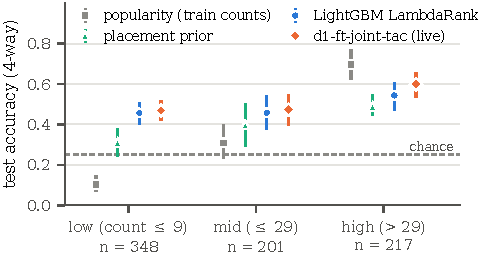
\includegraphics[width=\columnwidth]{figs/fig_popularity.pdf}
\caption{Test accuracy by training frequency of the gold key (terciles; 95\% cluster-bootstrap CIs). Popularity wins on head keys and fails on the tail; the fine-tuned LLM and LightGBM hold up on rare keys. Data: \tw{stats\_audit\_v1.json}.}
\label{fig:popularity}
\end{figure}

By training frequency of the gold key (Fig.~\ref{fig:popularity}), popularity is the best model on head keys (0.696) and the worst on the tail (0.103), while d1-ft-joint-tac and LightGBM stay level across the two lower terciles (0.468/0.473, 0.457/0.458), generalising beyond memorised keys; a share of 0.14 of test gold keys never occurs in training. % src: SA sec. 5

d1 is well calibrated (test ECE 0.048 over 15 bins; Brier 0.616): holding when its top probability is below 0.483 (chosen on val) answers 0.402 of test lines at 0.630 accuracy and raises the +1/0/$-$1 CRAG-style utility~\cite{yang2024cragbench} from 0.013 [$-$0.056, 0.079] to 0.104 [0.060, 0.147] (Fig.~\ref{fig:retsel}b). A d1+LightGBM ensemble changes test accuracy by $-$0.1, +2.1 or +3.9 points depending on LightGBM's seed, so we do not claim it; a rule arbiter narrowing d1's options when it is unsure gives no gain (0.509 vs 0.506) and stays off. % src: SA sec. 3, 4, 6; arbiter_v2.md (50.6% / 50.9%)

\subsection{Decision models}
\label{sec:decmodels}

\begin{table}[t]
\caption{Decision models on the 766 test lines of Table~\ref{tab:ranker} (game-bootstrap CIs, seed 0; d1's 0.5065 shows there as 0.507); middle block zero-shot. All differ from d1-ft-joint-tac at McNemar $p<0.001$ but LightGBM ($p=0.263$). $^\dagger$Thinking \tw{between\_tools}, $\le$2,000 output tokens, answer parsed from the end; with the 16-token cap of the other API runs 62.8\% of Sonnet replies were cut off (accuracy 0.144), 3.8\% of Haiku's (counted wrong).}
\label{tab:decmodels}
\centering\scriptsize
\setlength{\tabcolsep}{2.2pt}
\begin{tabular}{@{}llccc@{}}
\toprule
Model & Accuracy [95\% CI] & Card & ms p50/p95 & US\$/dec.\\
\midrule
\textbf{d1-ft-joint-tac}, 600M (live) & \textbf{0.506} [0.473, 0.538] & 0.692 & 75/117 & 0\\
d1-2B fine-tuned, 1.9B & 0.429 [0.394, 0.466] & 0.614 & 295/465 & 0\\
\midrule
d1-omni-600M zero-shot & 0.260 [0.235, 0.283] & 0.513 & 73/113 & 0\\
Qwen3-4B-Instruct-2507 & 0.286 [0.244, 0.331] & 0.527 & 802/1119 & 0\\
\quad + 3 retrieved pro states & 0.283 [0.251, 0.316] & 0.516 & 1535/1958 & 0\\
Qwen3-14B & 0.304 [0.264, 0.345] & 0.523 & 2721/3866 & 0\\
Claude Haiku 5.5 & 0.279 [0.250, 0.310] & 0.499 & 676/823 & 0.00009\\
Claude Sonnet 5.5$^\dagger$ & 0.364 [0.325, 0.403] & 0.585 & 2467/4824 & 0.00369\\
\midrule
LightGBM LambdaRank & 0.482 [0.448, 0.514] & 0.677 & 0.4/0.5 & 0\\
placement prior & 0.384 [0.336, 0.431] & 0.614 & 0.003/0.003 & 0\\
popularity & 0.325 [0.280, 0.373] & 0.453 & 0.001/0.002 & 0\\
random, one draw (exp.\ 0.250) & 0.269 [0.237, 0.301] & 0.539 & 0.001/0.001 & 0\\
\bottomrule
\end{tabular}
\end{table}
% src (Table decmodels): docs/data/decision_models_v1.md "Accuracy and latency" (every cell; Sonnet row = claude-sonnet-5-5-long,
%   the claude-sonnet-5-5 row gives 0.144 and 481/766 = 62.8% parse failures; Haiku 29/766 = 3.8%; random (expected) 0.250 / 0.500);
%   decision_models_v1.json models.d1-ft-joint-tac.acc.est = 0.5065, models.lightgbm.vs_reference.mcnemar_p = 0.26333;
%   Sonnet settings and "max_tokens" errors: tools/eval/bench_claude_rankers.py VARIANTS, runs/bench/au/preds/claude-*.jsonl

\emph{Protocol} (MAC-AU). The LLMs share one prompt: d1's input (state text with \tw{tactics:} and \tw{KG:} lines, options A--D with notes) and a request for the pro's choice. Qwen3~\cite{qwen2025qwen3} decodes greedily, Claude Haiku with 16 output tokens, both thinking off (Sonnet: $^\dagger$); the RAG variant prepends the 3 nearest train-split pro states (600 characters each, plus the pro's play). Latency is wall time per decision after a warm-up (M5: d1 on MPS, Qwen in MLX 4-bit, one model at a time; API: with the network); cost is usage times list price. % src: docs/plans/MAC-AU_decision_models_retrieval_benchmark.md (Part A prompt, Qwen, RAG, Claude, GPU discipline, Amendment 1); tools/eval/bench_llm_rankers.py (greedy, 8 new tokens, enable_thinking False); decision_models_v1.md header (latency definition)

\emph{Findings.} Fine-tuning dominates. Zero-shot, d1-omni-600M, both Qwen3 models and Claude Haiku 5.5 stay within 5.4 points of chance, the parametric-memory limit~\cite{mallen2023popqa,lim2026l11} (d1: 0.260 with notes, 0.221 without, Table~\ref{tab:ranker}). Claude Sonnet 5.5, the best zero-shot model, is 14.2 points [$-$19.1, $-$9.3] below the fine-tuned 600M at 33$\times$ its median latency and a per-decision cost: RankGPT-style zero-shot ranking~\cite{sun2023rankgpt,cap6938L10} falls short in this domain and budget. Three retrieved pro examples (RAG few-shot~\cite{lim2026l11}) do not help Qwen3-4B (0.283 vs 0.286) and nearly double its latency. The larger fine-tune is worse: d1-2B (top 8 layers trained, val 0.4192) loses 7.7 points [$-$12.2, $-$3.4] at 4$\times$ latency. LightGBM, a tuned baseline~\cite{rendle2020ncfvsmf,lim2026l13}, is on par at 0.4\,ms. % src: decision_models_v1.md (accuracies; diff column: Sonnet-long -0.142 [-0.191, -0.093], d1-2B -0.077 [-0.122, -0.034], LightGBM -0.025 [-0.059, +0.014]; latency p50 2467 / 75 = 33x, 295 / 75 = 3.9x, 1535 / 802 = 1.9x); 0.304 - 0.25 = 5.4 pts (Qwen3-14B, largest of the four); CMA C4 (d1-2B top 8 layers, val 0.4192); SA sec. 1 (0.221); CMA A2 parametric-memory row (d1_zero_shot_v1.json joint = plain lines, 0.2206 test)

\subsection{Retrieval}
\label{sec:retr}

\begin{table}[t]
\caption{Retrieval channels (916/902 val/test queries, train pool, depth 50). Hit@10: the pro's exact play is among the top-10 neighbours' plays.}
\label{tab:retrieval}
\centering\scriptsize
\setlength{\tabcolsep}{3pt}
\begin{tabular}{@{}lccc@{}}
\toprule
List & hit@10 val / test & card hit@10 val / test & ms p50 (test)\\
\midrule
BM25 (FTS5) & 0.142 / 0.159 & 0.396 / 0.483 & 25.8\\
structured kNN (644-d) & 0.166 / 0.136 & 0.434 / 0.412 & 2.1\\
text (bge-small, 384-d) & 0.132 / 0.143 & 0.397 / 0.436 & 22.2\\
struct + BM25 (live) & 0.138 / 0.160 & 0.434 / 0.487 & 28.0\\
all three, RRF & 0.156 / 0.170 & 0.461 / 0.514 & 49.6\\
\bottomrule
\end{tabular}
\end{table}
% src (Table retrieval): docs/data/retrieval_ablation_v1.md (kept current per BM sec. 3)

Table~\ref{tab:retrieval}: the channels are within noise (test hit@10 0.136--0.170); BM25 beats the structured channel on test (0.159 vs 0.136) but not on val, and the text channel adds about 20\,ms for no clear gain, so the live list is structured plus BM25. As a lone candidate source, kNN voting loses to popularity on exact keys (test recall@10 0.317 vs 0.402) and wins only on cards (0.651 vs 0.607). % src: CMA A1 (ranker_baselines_v1.json candidate_recall)
HNSW at ef 40 keeps recall@10 at 0.978 in 0.31 vs 1.51\,ms for exact search (Fig.~\ref{fig:retsel}a), but at 10.9k vectors exact search stays live. For pre- vs post-filtering~\cite{cap6938L09}, a deck pre-filter empties the pool for 88.9\% of queries (decks unseen in training); post-filtering the top 10 returns nothing for 50.0\% (deck) and 87.3\% (phase) of queries, the top 200 for 0.5\% and 0.1\%. % src: retrieval_ablation_v1.md (HNSW table, filtering table)

\begin{figure}[t]
\centering
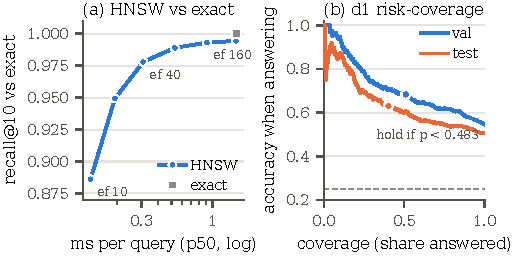
\includegraphics[width=\columnwidth]{figs/fig_retrieval_selective.pdf}
\caption{(a) HNSW recall@10 against exact kNN versus query time (10,923 vectors, $k{=}10$). (b) Risk--coverage of d1-ft-joint-tac holding below a probability threshold (dots: 0.483, set on val).}
\label{fig:retsel}
\end{figure}

\subsection{KG embeddings and mined rules}
\label{sec:kg}

\begin{table}[t]
\caption{Held-out COUNTERS link prediction, test (762 queries, filtered, 3 seeds).}
\label{tab:kg}
\centering\scriptsize
\setlength{\tabcolsep}{3pt}
\begin{tabular}{@{}lccc@{}}
\toprule
Method & MRR & H@1 & H@10\\
\midrule
random & 0.0223 & 0.0113 & 0.1129\\
popularity & 0.1103 & 0.0381 & 0.2385\\
TransE & 0.0819 $\pm$ 0.0046 & 0.0000 & 0.2380\\
DistMult & 0.0907 $\pm$ 0.0083 & 0.0232 & 0.1986\\
ComplEx & 0.1162 $\pm$ 0.0074 & 0.0367 & 0.2616\\
RotatE & \textbf{0.1588} $\pm$ 0.0020 & 0.0713 & 0.3259\\
\bottomrule
\end{tabular}
\end{table}
% src (Table kg): docs/data/kge_link_prediction_v1.md (setting full). The former part (b), E6 test hit@1 / MRR, is identical to Table retrmethods (b)
%   rows v2 full / pro only / v1 wiki COUNTERS / popularity / random (answer_rules_v1.md test table = retrieval_methods_v1.md KG table)

\emph{Link prediction} (Table~\ref{tab:kg}). We hold out wiki COUNTERS triples (3,043/380/381) and rank 126 candidate cards (filtered, tie-aware); all four PyKEEN~\cite{ali2021pykeen} models get the same grid (dimension 32 or 64, learning rate 0.01 or 0.001; chosen on val MRR) and three seeds, per the course's evaluation-audit protocol~\cite{ruffinelli2020olddog,sun2020reevaluation,cap6938L05}. RotatE~\cite{sun2019rotate} is best and beats popularity; TransE and DistMult do not, DistMult being symmetric by construction (asymmetry score 0.0) while only 940 of 3,804 counter pairs have a reverse edge. % src: CMA A3 (triples, grid, asymmetry, 940 / 3,804); kge_link_prediction_v1.md

\emph{Mined answer rules} (E6; test in Table~\ref{tab:retrmethods}b). For each of 609/433 held-out val/test events we rank the pro's own deck (7.96/7.83 cards on average) with rules mined from training games (support $\ge3$, 8\,s window); val hit@1: full 0.182, pro-mined only 0.191, wiki COUNTERS 0.117, train popularity 0.182, random 0.126. Pooled over val and test, the full score beats random (+0.044 hit@1 [+0.020, +0.068]) and the wiki counters (+0.043 [+0.011, +0.074]) but not the training popularity of the answer card ($-$0.006 [$-$0.035, +0.020]); on test the pro-mined source alone falls below popularity ($-$0.040 hit@1, $p=0.022$). The score barely predicts whether the answer held the tower (AUROC 0.543), few rules have large support (10 or more for 63 of 1,042 events), and 8\,s is the best window of 2, 4 and 8\,s on val (MRR 0.409). Unlike AMIE and TLogic, which score rules on their mining data~\cite{lajus2020amie3,liu2022tlogic}, this held-out test against popularity~\cite{ruffinelli2020olddog} shows the 287 rules mostly re-encode the pro's card frequencies, a weak prior~\cite{cap6938L07}. % src: answer_rules_v1.md (headline val table: 0.182, 0.191, 0.117, 0.182, 0.126; 609 / 433 events; paired val+test, test paired, AUROC, strata, sweep)

\subsection{Retrieval methods for the KB and the KG}
\label{sec:retrmethods}

\begin{table}[t]
\caption{KB and KG methods on the 766 test lines, retrieving from train games. (a)~KB, top 20: a hit's pro play has the gold key (hit@10, MRR) or card (card@10); rec.\ = overlap with exact top 20. (b)~KG: 433 held-out threat$\rightarrow$answer events, ranked over the pro's deck. 4-way: accuracy as a decision model (unsupported lines tied); Cov.: share of lines supported; ms: query p50. Two options share each card: a card-level score is capped at 0.5 4-way.}
\label{tab:retrmethods}
\centering\scriptsize
\setlength{\tabcolsep}{2.4pt}
\begin{tabular}{@{}lcccccc@{}}
\toprule
(a) KB method & hit@10 & card@10 & MRR & 4-way & Cov. & ms\\
\midrule
dense exact (644-d, dot) & 0.144 & 0.423 & 0.067 & 0.284 & 0.53 & 1.16\\
BM25 (FTS5) & 0.166 & 0.491 & 0.060 & \textbf{0.318} & 0.53 & 22.14\\
RRF dense + BM25 (live) & 0.175 & 0.501 & 0.074 & 0.305 & 0.58 & 24.19\\
bge-small text (cosine) & 0.155 & 0.450 & 0.067 & 0.307 & 0.46 & 13.64\\
RRF all three & \textbf{0.184} & \textbf{0.530} & \textbf{0.082} & 0.314 & 0.54 & 45.16\\
HNSW ef 10 (rec.\ 0.977) & 0.141 & 0.418 & 0.067 & 0.287 & 0.52 & 0.84\\
HNSW ef 40 (rec.\ 0.990) & 0.141 & 0.419 & 0.067 & 0.286 & 0.53 & 1.11\\
HNSW ef 160 (rec.\ 0.998) & 0.142 & 0.422 & 0.067 & 0.286 & 0.53 & 2.24\\
deck pre-filter, then dense & 0.076 & 0.157 & 0.041 & 0.286 & 0.16 & 0.82\\
\midrule
(b) KG method & hit@1 & hit@3 & MRR & 4-way & Cov. & ms\\
\midrule
v1 \tw{counter\_scores} & 0.143 & 0.409 & 0.360 & 0.249 & 0.31 & 0.01\\
v1 wiki COUNTERS only & 0.141 & 0.406 & 0.359 & 0.250 & 0.29 & 0.01\\
v2 \tw{answers\_for}, full & 0.154 & 0.422 & 0.374 & 0.239 & 0.45 & 0.05\\
\quad pro source only & 0.129 & 0.399 & 0.350 & 0.236 & 0.20 & 0.04\\
\quad role transfer only & 0.145 & 0.398 & 0.356 & 0.241 & 0.24 & 0.04\\
\quad wiki only & 0.147 & 0.407 & 0.362 & 0.249 & 0.29 & 0.04\\
\quad simulation (STOPS) only & 0.157 & \textbf{0.440} & 0.376 & \textbf{0.258} & 0.31 & 0.04\\
KGE RotatE & 0.125 & 0.400 & 0.340 & 0.253 & 0.49 & 0.18\\
KGE TransE & 0.118 & 0.353 & 0.335 & 0.245 & 0.49 & 0.13\\
train popularity of the answer & \textbf{0.169} & 0.433 & \textbf{0.384} & 0.217 & 0.49 & 0.00\\
random (expected) & 0.128 & 0.384 & 0.345 & 0.250 & -- & --\\
\bottomrule
\end{tabular}
\end{table}
% src (Table retrmethods): docs/data/retrieval_methods_v1.md, "KB: the pro-state database" (hit@10, card_hit@10, MRR, 4-way acc,
%   coverage, recall@20 vs exact, ms p50) and "KG: threat to answer" (hit@1, hit@3, MRR, 4-way acc, line coverage, query ms p50);
%   433 events / 374 lines with a threat, train-only pool and leak check, card-level cap 0.5: same file, "Setup and leakage"

As retrievers (Table~\ref{tab:retrmethods}a) the hybrids lead (\cf Sec.~\ref{sec:retr} and~\cite{cap6938L08,cap6938L09,cap6938L10}): RRF of all three lists has the best hit@10, card@10 and MRR, and the live dense+BM25 fusion beats both its lists (hit@10 0.175 vs 0.144, 0.166), with overlapping CIs. HNSW keeps 0.977--0.998 of the exact top 20, but over 4,997 train states exact search takes only 1.16\,ms (ef 10 saves 0.3\,ms). The deck pre-filter returns nothing for 78.3\% of lines (decks unseen in train; the pre-filter risk of~\cite{cap6938L09}), though on the 16\% it supports it is the most accurate KB rule (0.475). % src: retrieval_methods_v1.md KB table (recall@20, ms, empty 0.783, acc if supported 0.475 [0.312, 0.587]) and Setup (4,997 train states with an action); 1.16 - 0.84 = 0.32 ms
No method alone is a usable decision maker: the best, BM25, reaches 0.318 [0.283, 0.351], 18.9 points below d1, other KB methods 19--22 and the KG methods 25--29 points below (all McNemar $p<10^{-12}$), as a card-level score cannot place and finds a threat on 374 of 766 lines; no KG method beats train popularity on hit@1 or MRR (0.169, 0.384). Their value is as candidate sources and ranker context (Sec.~\ref{sec:disc}). % src: retrieval_methods_v1.md "Retrieval as a decision model" (delta vs d1: KB -0.189 to -0.222, KG -0.248 to -0.289; largest McNemar p 2.28e-13), Headline (BM25 0.318 [0.283, 0.351]; popularity MRR 0.384)

\subsection{Context conflict: does d1 follow notes? (E2)}
\label{sec:conflict}

Following ClashEval and the knowledge-conflict lecture~\cite{wu2024clasheval,xie2024chameleon,lim2026l17}, we corrupt d1-ft-joint-tac's context with the gold label fixed: C1 removes the notes and \tw{tactics:}/\tw{KG:} lines; C2 shuffles the notes across options; C3 swaps the gold option's informative note with a distractor's and names a wrong card in the \tw{tactics:} line (relevant but misleading); C4 transplants another line's tactics/KG block (irrelevant). Follow-rate: the share of movable lines (the corruption favours an option d1 did not pick) whose pick moves to the favoured option.

\begin{table}[t]
\caption{Context conflict on d1-ft-joint-tac (E2), test lines (n = 766, 27 games), 95\% cluster-bootstrap CI; $p$ = exact McNemar; follow-rate as in the text (C4: 12 movable lines).}
\label{tab:conflict}
\centering\scriptsize
\setlength{\tabcolsep}{3pt}
\begin{tabular}{@{}lllcc@{}}
\toprule
Condition & Accuracy [CI] & $\Delta$ pts ($p$) & Changed & Follow\\
\midrule
C0 as exported & 0.507 [0.473, 0.539] & -- & -- & --\\
C1 context removed & 0.508 [0.476, 0.541] & +0.1 (1.00) & 21\% & --\\
C2 notes shuffled & 0.517 [0.482, 0.550] & +1.0 (0.27) & 7\% & 0.094\\
C3 notes poisoned & 0.503 [0.469, 0.535] & $-$0.4 (0.76) & 6\% & 0.044\\
C4 block transplanted & 0.495 [0.459, 0.530] & $-$1.2 (0.45) & 19\% & 0.083\\
\bottomrule
\end{tabular}
\end{table}
% src (Table conflict): docs/data/context_conflict_v1.md, replicate on joint_tac_v2 (HEAD notes, same lines as Table III), "Accuracy by condition - test" and "Follow-rate - test"; p = exact McNemar

Table~\ref{tab:conflict}: no condition moves accuracy by more than 1.2 points. Removing the whole context changes 21\% of picks, but gains and losses cancel (57 vs 56 lines); poisoned notes move 4.4\% [2.1, 6.8] of movable picks. Lines whose gold option carries the informative note are easier than lines where a distractor's does (0.564 vs 0.371), but the gap persists with no notes (0.599 vs 0.401), so it reflects which states are easy. Context-aware decoding~\cite{shi2024cad} selects weight $a=0$ on val in every condition, and each $a>0$ lowers C0 test accuracy by 1.7 to 2.9 points; AdaCAD's adaptive weight~\cite{wang2025adacad} averages 0.014 and changes accuracy by $-$0.1 points. % src: CC replicate joint_tac_v2 (test tables, strata, CAD C0)
d1 thus avoids both failures the course warns about, adopting wrong context over its prior (ClashEval~\cite{wu2024clasheval}) and greater sensitivity to relevant-but-misleading than to irrelevant noise (RAGChecker~\cite{ru2024ragchecker}), because it barely reads its notes, plausibly as they favour the gold option on only 30\% of test lines and a distractor on 22\% (49\% have none), so it is robust to wrong tool output. % src: CC replicate test note status (227 right, 167 wrong, 372 none of 766)

\subsection{When to act}
\label{sec:timing}

On dense test seconds (n = 5,279), balanced accuracy for ``the pro deploys within $h$'' at $h$ = 1/2/3\,s is 0.506/0.509/0.510 for the hand-written rules and 0.594/\textbf{0.607}/0.613 for LightGBM on 29 features (AUC 0.632/0.659/0.672); the live \emph{fast} combination, with rules overriding the model in four modes, sits between them (0.571/0.584/0.593). % src (Table timing): docs/data/act_gbdt_v2.md overview + apples-to-apples test table; act_head_v2.md (0.558, unchanged from v1)
On the balanced subset ($h=1$\,s, n = 3,221) used to train a d1 act head (top 8 layers, 168.9M trainable parameters), LightGBM scores 0.598 against the head's 0.558, at 0.05\,ms instead of about 70\,ms per call: again the tuned simple model beats the LLM. % src: act_gbdt_v2.md (apples-to-apples test table); act_head_v2.md (0.558); CMA B (act head 168.9M, ~70 ms), C4

\subsection{Next card, opponent deck, knowledge editing}

For opponent next-card prediction, a sequential recommendation task~\cite{kang2018sasrec,lim2026l14}, SASRec (3 seeds) reaches acc@1 0.129/0.222 on val/test and loses to a copy-frequency rule (0.207/0.243), the copy intuition of CyGNet~\cite{zhu2021cygnet,cap6938L06C}; popularity is near zero (0.000/0.002) because opponents vary, and the ceiling set by cards already seen is 0.678/0.644. The KG opponent-deck model recovers hidden cards with recall 0.234/0.291/0.327 after 1/2/3 seen cards, against 0.130/0.124/0.118 for popularity (leave-one-game-out, 155 games). % src: next_card_v1.md; opp_model_v1.md (BM sec. 7)
For knowledge editing~\cite{yao2023editingsurvey,lim2026l17} we apply a synthetic +1-elixir patch to five cards in a patch-versioned fact store, SERAC's non-parametric route~\cite{mitchell2022serac}: reliability, generalisation and portability are 1.000 (0.000, 0.000, 0.067 without the edit), locality 1.000, rollback passes, and re-weighting cuts retrieved hits using an edited card from 0.124 to 0.002; the store is deterministic, so this shows the mechanism, not that it generalises to a real patch~\cite{yang2025mirage}. % src: edit_eval_v2.md (identical to edit_eval_v1.md)

\subsection{Bot versus pro on held-out videos}

We run the live stack open loop on held-out test videos with the pro's deck and a dry-run executor, matching its would-be taps to the pro's plays within $\pm$2\,s. As taps do not change the video, this measures what the bot would do in the pro's place, not whether it would win (its hand memory never learns a card left the hand). Retrieval uses only train and val games, the KG answers and placement prior only train games. Results cover the 24 usable test games (90\,min, 1,561 pro plays, 2,042 bot taps); 4 more lack a full deck. % src: VP header and "Not run" list

\begin{table}[t]
\caption{Bot vs pro on held-out pro videos, open loop: 24 test games, 1,561 pro plays. Percent; window $\pm$2\,s; 95\% CIs by game bootstrap. Null: the bot's own taps shifted by 20--60\,s. Baselines use the same plays; the placement prior is given the pro's card.}
\label{tab:vspro}
\centering\scriptsize
\setlength{\tabcolsep}{3pt}
\begin{tabular}{@{}lll@{}}
\toprule
Measure & Bot [95\% CI] & Baseline\\
\midrule
pro plays met by a bot tap & 77.1 [71.8, 83.0] & 68.9 (null)\\
bot taps met by a pro play & 72.6 [69.3, 76.2] & 67.9 (null)\\
taps (bot) / plays (pro) per min & 22.8 [20.2, 25.9] & 17.4 [16.5, 18.4]\\
same card, matched pairs & 17.1 [14.6, 20.2] & 12.8 (random in hand)\\
same card, KG threat exists (126) & 19.8 [13.3, 26.9] & 15.6 (KG v1 counter)\\
pro's card in perceived hand & 40.1 [37.3, 43.2] & 53.0 (dataset's hand)\\
same lane $\mid$ same card (103) & 42.7 [31.6, 53.5] & 44.6 (placement prior)\\
same key $\mid$ same card (103) & 26.2 [16.8, 36.0] & 29.7 (placement prior)\\
\bottomrule
\end{tabular}
\end{table}
% src (Table vspro): docs/data/vs_pro_v1.md (MAC-AQ, generated 2026-11-08T02:31:35Z, all 24 usable test games) Headline table (every cell, subset sizes 126 and 103) and Timing table.

Table~\ref{tab:vspro}: the bot's timing beats the null (matched taps a median 0.47\,s from the pro's play), which matters because it taps more often and spends more elixir than the pro (58.7 vs 33.6 per minute). Its card choice beats a random card of its hand and, where a KG threat exists, the KG v1 counter rule, but the ceiling is low: the pro's card is in the perceived hand on only 40.1\% of plays, and the bot cannot pick a card it does not see. Missed pro plays were mostly held because no card was affordable (23.0\%), the engine left the push to the tower (22.7\%) or the act model waited (18.8\%). % src: VP Headline, Timing (0.47 s; elixir/min 58.72, 33.58), When the bot held

\subsection{Live play and prior bots}
\label{sec:live}

\begin{table}[t]
\caption{(a) Latency by stage, ms p50 / p95: live trial session (363 decisions) and mean of 3 video dry runs ($\pm$ sd for the total; a shared Mac, so upper bounds). (b) Live record in Training Camp.}
\label{tab:live}
\centering\scriptsize
\setlength{\tabcolsep}{3pt}
\begin{tabular}{@{}lcc@{}}
\toprule
(a) Stage & trial session & dry run, 3 reps\\
\midrule
capture & 22.0 / 44.8 & 0.8 / 4.3\\
perception (detector, OCR, hand) & 108.0 / 266.4 & 179.2 / 234.2\\
live state & 0.13 / 0.31 & 0.2 / 0.5\\
trigger (rules + LightGBM) & 1.1 / 9.2 & 2.7 / 9.7\\
candidates (engine, retrieval, KG) & 26.8 / 57.9 & 46.7 / 86.1\\
rank (d1; 0 when one candidate) & 0.0 / 140.9 & 87.1 / 191.0\\
execute (two clicks) & 181.0 / 188.8 & no clicks\\
\textbf{total} & \textbf{322.7 / 601.6} & 271.7$\pm$20.1 / 455.2$\pm$41.2\\
\midrule
\multicolumn{3}{@{}l}{(b) Live record}\\
\midrule
runs before the trial, 11-03 to 11-07 & \multicolumn{2}{l}{13 (12 live), 931 decisions, 746 taps}\\
taps landed, two newest of them & \multicolumn{2}{l}{75/84, 78/95 (older run 233907: 95/100)}\\
run 013441 (3 battles) & \multicolumn{2}{l}{tower taken; 3-crown loss; \textbf{win in overtime}}\\
\textbf{trial}: wins / battles, exact CI & \multicolumn{2}{l}{\textbf{0 / 10}, 95\% CI 0--30.8\%}\\
\quad crowns for / against (10 battles) & \multicolumn{2}{l}{3 / 18; a tower taken in 3; 2 in overtime}\\
\quad per logged battle (9 of 10) & \multicolumn{2}{l}{40.3 decisions, 27.0 taps; median 213\,s}\\
\bottomrule
\end{tabular}
\end{table}
% src (Table live): (a) trial-session column: LOG decisions.jsonl timings_ms, all 363 rows, nearest-rank p50 / p95 (total 322.7 / 601.6);
%   dry-run column: LAT "Whole stack, 3 repeated dry runs" (video Z8-4VhLjrGU 60-180 s, runs/rerun/lat_{1,2,3}), mean of p50 / p95, sd for total
%   (b) CMA C6 = BM sec. 13 (12 live runs, 931, 746) + LAT (dry run 20261105-205720); BM sec. 11 (tap_landing_20261107-013441_v2.md 75/84,
%   tap_landing_20261107-111554_v2.md 78/95, tap_landing_233907_v1.md 95/100); STATUS 2026-11-07 night (run 013441);
%   trial rows: TRIAL (0/10, scores, crowns 3/18, 2 OT, 3 with a tower; Clopper-Pearson 0-30.8%, checked with scipy beta.ppf(0.975,1,10) = 0.3085);
%   LOG battles.jsonl (9 TRAINING_CAMP rows: 363 decisions, 243 taps, median duration 212.6 s) and decisions.jsonl timings_ms (total 323/602)

The 13 runs before the trial (Table~\ref{tab:live}b; 12 live, one dry) took 347/613\,ms p50/p95 in total (339/572\,ms in run 111554). In the trial (Table~\ref{tab:live}a) perception (108\,ms p50) and the two-click execute stage (181\,ms) dominate; d1 adds nothing at the median, as most decisions have one candidate, and 141\,ms at p95. The 300\,ms p95 target was missed in every live run and all three dry runs. Failed taps concentrate on Tesla (11 of 19 landed in run 111554) and Fireball (3 of 7). % src: CMA C6, C7 (347/613; 338.9/571.8 run 111554); LOG (trial session); LAT (dry runs: 0 of 3 meet the target); BM header (shared Mac); tap_landing_20261107-111554_v2.md (tesla 11/19, fireball 3/7); STATUS 2026-11-07 night
\emph{Trial.} On 2026-11-07 ten Training Camp battles were played through the launcher (\tw{scripts/demo.sh --live}) on the frozen code (D-051), results recorded by hand. All ten were lost (Table~\ref{tab:live}b): 0--1 five times (once in overtime), 0--2, 0--3, 1--2, and 1--3 twice (once in overtime); against KataCR's 1/20 a two-sided Fisher exact test gives $p=1.0$. The session log holds 9 of the 10 battles (one start was missed), and the banner gate correctly refused two non-battle screens whose banner read ``2618''. % src: TRIAL (scores, Fisher p = 1.0 checked with scipy fisher_exact [[0,10],[1,19]]); LOG (decisions.jsonl timings_ms; battles.jsonl n = 2, 3 banner "2618" NOT_TRAINING_CAMP)

\begin{table}[t]
\caption{Prior Clash Royale agents and \cb{}. R = reported by the authors, M = measured by us. Protocols differ; see text.}
\label{tab:prior}
\centering\scriptsize
\setlength{\tabcolsep}{2pt}
\begin{tabular}{@{}L{1.18cm}L{2.35cm}L{1.72cm}L{2.6cm}@{}}
\toprule
 & KataCR~\cite{wu2025nonembedded} & Claude Royale~\cite{houseworth2025claudeRoyale} & \cb{} (ours)\\
\midrule
Interface & video stream, ADB taps (Linux) & BlueStacks (macOS) & iPhone Mirroring, Quartz clicks (macOS)\\
Perception & YOLOv8-l$\times$2 (mAP 67.4), OCR, ResNet classifiers & Claude vision & KataCR's YOLOv8 weights, OCR, Kalman tracker\\
Decision & offline-RL StARformer & Claude Haiku, 3 agents & gate, engine, retrieval, KG; fine-tuned 600M LLM picks\\
Knowledge used & none (in weights) & hand-written prompts, notes & 10,923 pro states, KG v1/v2, tactics engine\\
Training data & 105 episodes, 113,981 frames, one player vs AI & none (prompting) & 197 pro games, 33 videos\\
Latency & 120\,ms decision + 240\,ms fusion (R) & $\sim$7\,s per agent (R) & 323/602\,ms p50/p95, capture to click, trial (M)\\
Offline metric & none & card choice 11/25 on labelled screenshots (R) & 4-way test accuracy 0.507 (M)\\
Opponent & built-in AI (Training Camp) & human ladder & built-in AI (Training Camp)\\
Win rate, 95\% CI & 1/20 = 5\% [0.1, 24.9]; 0--10\% over 9 models (R) & none (ladder; not comparable) & trial 0/10 [0, 30.8]; one earlier win (M)\\
\bottomrule
\end{tabular}
\end{table}
% src (Table prior): PBC sec. 0, 1.2-1.4, 2.1-2.2, 4, 5 (Clopper-Pearson 1/20: 0.1-24.9%); ours CMA C7, SA sec. 1; TRIAL (0/10, CI, Fisher); STATUS 2026-11-07 night (earlier win)

Table~\ref{tab:prior}: only KataCR and \cb{} report a win rate against the built-in AI, under different protocols: KataCR played the 2024 game (Season 59) with another deck, and its 1/20 is the best of ten epochs selected on the same 20 games (optimistic); its latency excludes actuation, ours includes it. We reuse its detector and claim no better one. % src: PBC sec. 5, 6

\section{Discussion and Limitations}
\label{sec:disc}

Four results are negative, and each repeats a course lesson. \emph{Tuned simple baselines match the LLM} on ranking and timing (Sec.~\ref{sec:ranker}, \ref{sec:decmodels}, \ref{sec:timing}), and copy-frequency beats SASRec: well-tuned simple models often match neural ones~\cite{rendle2020ncfvsmf,lim2026l13}, and 197 games from one creator leave a 600M model little to learn beyond the priors a GBDT reads directly. % src: SA sec. 2; feature_ranker_v2.md; act_gbdt_v2.md; next_card_v1.md
\emph{d1 does not read its context} (Sec.~\ref{sec:conflict}), the opposite extreme from the over-trusting models of~\cite{wu2024clasheval,ru2024ragchecker}; with the engine near chance as a ranker (4-way 0.293/0.265 val/test), the tools contribute by proposing candidates, not by writing notes~\cite{lim2026l13}. % src: CC replicate; tactics_eval_v2.md
\emph{Mined rules approximate popularity} (Sec.~\ref{sec:kg}): the evaluation audits the course teaches~\cite{ruffinelli2020olddog,sun2020reevaluation} ask for exactly this baseline (the protocol matters as much as the method), and the same habit caught the option-set leak before d1 was fine-tuned on it (D-037). % src: D-037 (2026-11-02) precedes D-039 (fine-tune go-ahead, 2026-11-03)
\emph{Perception caps agreement with the pro}: besides the 40.1\% hand ceiling and the 0.542--0.597 legality rate, in an early live run 14 of 27 decisions were skipped because the hand read as unknown. As the ESCA lecture argues, perception errors dominate embodied-agent failures~\cite{huang2025esca,cap6938L06C}. % src: VP headline (40.1); CMA A3 (0.542-0.597); BM sec. 13 and PBA 2.2 (14 of 27; CMA A3 says 15 of 27)

\emph{Why the trial was lost (limitations and future work).} (1)~\emph{Tower HP:} OCR drops digits (one tower read 4424$\leftrightarrow$424 seven times in 30\,s) and a fallen tower reads unknown, not 0, so the deploy area it opens went unused (a tower fell in 3 battles). (2)~\emph{No committed target:} counter-pushes follow the defended push's lane, splitting damage (one battle ended with enemy towers at 1,663 and 1,824 HP, neither taken), and after a tower fell ram riders kept taking its lane, \ie went at the king. (3)~\emph{No support} troop is offered behind a surviving defence or a ram rider. (4)~\emph{Spell value:} Fireball is valued by elixir destroyed, not tower damage prevented, so none was proposed against a bunched Giant, Balloon and Bats push, and the Zap group rule counts tanks. (5)~\emph{Over-playing:} 27 taps per battle, 40 emergency defends at 2--5 elixir and 30 tap pairs under 1.6\,s apart, as on video (Table~\ref{tab:vspro}). (6)~\emph{Phantom threats:} a stationary ``Graveyard'', a card the trainer's deck lacks, triggered defences six times. All six sit in the hand-written engine and policy, which our benchmarks rate lowest (timing rules 0.509 balanced accuracy, the engine 0.265 as a ranker), and d1 cannot repair them: it ranks only when two or more candidates survive (119 of 279 executed plays) and ignores the notes. Fixes (monotone HP filter, per-battle target tower, pocket placements, support moves, spell value from prevented damage, elixir budget at the pro's rate) are specified for a re-run against this 0/10 baseline. % src: BL W1 (B1 4424/424 x7, t 41-70), W3 (legal_zones needs 0), W2 (B4 1663/1824; B8 ram riders right after the right tower fell), W4, W5 (B9 giant+balloon+bats, value by elixir), W6 (group rule counts the giant), W8 (243 taps / 9 battles; 40 emergency defends 2-5 elixir), W9 (30 pairs < 1.6 s), W10 (graveyard x6, not in Trainer Cheddar's deck); VP (22.8 vs 17.4; "no affordable card" 23.0%); act_gbdt_v2.md (0.509); tactics_eval_v2.md (0.265); CMA sec. 0 (119/279)

\emph{Other limitations.} d1's serve-time context carries a \tw{[plan]} line no training line contains, an unmeasured train/serve mismatch. Every offline number rests on 26--27 held-out games from one creator, and three of our eight cards have no pro plays, so the engine and role transfer carry them. Video evaluation is open loop; perception ignores enemy health bars (units are simulated at full HP). Trial results were recorded by hand: the end-of-battle frames missed the result screen in 5 of 9 battles. % src: CMA sec. 0 ([plan]); SA sec. 1 (26/27 games); CGA sec. 7.3 E1 and PBA 2.4 (about +/-3.5 pts at n = 766); D-047 (ram-rider, electro-dragon, mini-pekka have no pro plays); STATUS MAC-AM merged (#57 full HP); d1-2B now tested (loader fix, decision_models_v1.md; Sec. decmodels); BL W11 (5 of 9)

\section{Conclusion}
\label{sec:concl}

\cb{} shows that a non-embedded agent can play Clash Royale live on a laptop, with knowledge-graph, retrieval and simulation tools feeding a fine-tuned LLM that keeps the final say, at 323\,ms from capture to click. Fine-tuning turned a chance-level LLM into one that picks the pro's play half the time, but tuned simple models match it, it ignores the tools' notes, and the agent does not yet beat Training Camp reliably (one early win, then 0/10). Next steps: fix the four trial failures of Sec.~\ref{sec:disc} (tower HP, target tower, spell value, over-playing) and re-run the 10-battle trial with automatic result logging, measure perception against labelled frames, and train d1 on lines where notes and leak-free KG facts carry signal the state lines do not. Code, tests, benchmark files (\tw{docs/data/BENCHMARKS.md}) and the decision log are in the project repository. % src: CMA C7; SA sec. 1; CC; AR; VP; PBA 2.5; TRIAL; BL (suggested order, W11)


{
    \small
    \bibliographystyle{ieeenat_fullname}
    \bibliography{main}
}

\end{document}
